\documentclass[../draft_1.tex]{subfiles}

\begin{document}

\chapter{Mathematical Ingredients}

We will begin this chapter by briefly introducing finite element methods and before particularly focusing on least squares finite element methods. The subsequent sections will then give a general overview of space-time solution methods, before going into more detail about the methodology applied in this thesis. Before finally discussing nonlinear iteration schemes. While these concepts or methods are introduced separately here, we will use chapter 4 to tie them together in a \textit{comprehensive} solver.


\section{Finite Element Methods}

In order to find a numerical estimate to the solution of a partial differential equation we need a way to approximate the operators involved. And while there are many different ideas of how to do so the one we have chosen to employ is a finite element approach, as they have shown to be one of the most powerful and versatile methodologies for the problem at hand \cite{bochev2009least}. The purpose of the subsequent section is not to establish the whole finite element framework from scratch but rather to provide the introduction of a unified notation that will be referred to throughout this thesis and a recollection of the most important properties needed. Anything else would be far beyond the scope this thesis, as a full description of the underlying mathematical constructions can quickly become rather involved but we would like to refer to \cite{evans2010partial} or \textit{[good finite element specific source?!]} for a comprehensive \textit{discussion} of the topic. 

%"a fem is first and foremost a quasi-projection scheme. ... approximate solutions are then characterized as quasi-projections of the exact (weak) solutions onto the closed subspace.

%FEM: do not directly deal with directly deal differential operators but through weak formulations leads to functional approximation as opposed to operator approximation

\subsection{General Setting}

The foundation of every finite element formulation is finding an appropriate weak formulation which includes the choice of suitable trial and solution spaces. This is especially applicable in the case of a least squares approach and will be discussed in further detail in section [...]. 

Given Banach spaces $X$ and $Y$, a bounded linear operator $\mathcal{A} : X \rightarrow Y$, $f \in Y$, we consider the problem:
\begin{ceqn}
\begin{align}
\text{Find } u \in X \text{ such that } \quad \mathcal{A} u = f \text{ in } Y.
\end{align}
\end{ceqn}

We are interested in the case where $\mathcal{A}$ represents a partial differential operator. As mentioned before the process of discretisation begins with turning (3.6) into a suitable variational equation which is defined in terms of two Hilbert spaces $V$ and $W$, a continuous bilinear form $a(\cdot, \cdot): V \times W \rightarrow \mathbb{R}$, and a bounded linear functional $L_f(\cdot): W \rightarrow \mathbb{R}$ and is given by
\begin{ceqn}
\begin{equation}
\begin{aligned}
\text{Find } u \text{ in } V \text{ such that:  } a(u, v) = L_f(v) \quad \forall v \in V
\end{aligned}
\end{equation}
\end{ceqn}
An operator equation such as (3.6) may be reformulated into several different variational equations. We can see that we were originally seeking for a solution $u$ in the space $X$ whereas in the weak formulation one attempts to find a solution in the space $V$, and which generally doesnt lie in $X$, and is therefore often referred to as a weak solution. Hence the relationship between the spaces $X, Y$ and $V, W$, and the operator $\mathcal{A}$ and the bilinear form $a(\cdot, \cdot)$ are of great importance, and while one generally wants the solution of the variational formulation (3.7) to be a "good" representation of the solution of the original problem (3.6), the definition of what that exactly means varies and usually depends on the nature of the problem and often some practicality issues. One possibility could be ... or too much? Therefore we have denoted them by the same letter but to be precise the solution $u$ appearing in the subsequent paragraphs will always be referring to $u \in V$, because our aim now is to solve the variational formulation.

So let us assume for now that we have found a suitable weak formulation of the operator equation where trial and test space are equal, that is $V = W$. In addition to $a(\cdot, \cdot)$ being linear and bounded, which is equivalent to the continuity, we will also require it to be symmetric, hence we have more specifically that
\bigskip
\\
$a(v_1, v_2) = a(v_2, v_1)$ for all  $v_1, v_2 \in V$ (symmetry) \\
$a(v_1, v_2) \leq \beta ||v_1||_V \cdot ||v_2||_V $, for all $v_1, v_2 \in V$ and $\beta > 0$ (boundedness) \\ $a(v_1, v_1) \geq \alpha ||v_1||_V^2$, for all $v_1 \in V$ and $\alpha > 0$ (coercivity)
\bigskip
\\
and $f \in V^*$, the dual space of $V$. Furthermore let us have homogeneous Dirichlet boundary conditions, that is $u = v = 0$ on $\partial \Omega$. Then by \textit{Riesz representation theorem/Lax-Milgram} we obtain that there exists a unique solution $u \in V$ that solves (2.2). And additionally the existence of an operator $\tilde{\mathcal{A}} : V \rightarrow V^*$ given by
\begin{ceqn}
\begin{align}
a(u,v) = \langle \tilde{\mathcal{A}} u, v \rangle_{V^*, V} \quad \forall u, v \in V
\end{align}
\end{ceqn}
where $\langle \cdot, \cdot \rangle$ denotes the duality pairing (more...) between $V$ and its dual space $V*$. Likewise we obtain for $L_f(\cdot)$ the existence of an unique (!) element $\tilde{f}$ through the relation
\begin{ceqn}
\begin{align}
L_f(v) = \langle \tilde{f}, v \rangle_{V^*, V} \quad \forall v \in V
\end{align} 
\end{ceqn}
The variational formulation is therefore equivalent to the problem 
\begin{ceqn}
\begin{align}
\text{Find } u \in V \text{ such that } \quad \tilde{\mathcal{A}} u = \tilde{f} \quad  \text{in } W^*
\end{align}
\end{ceqn}
In the special case that $X = U$ and $Y = W^*$ we have that $ \mathcal{A} = \tilde{\mathcal{A}}$ and $ f = \tilde{f}$ but this is generally not the case. 

\subsection{Discretisation}
A key element to actually finding a good approximation $u^h$ of $u$ is to choose a suitable finite dimensional (sub)space $V_h$ where we search for the solution. We will consider a \textit{Galerkin approach}, where we indeed have $V_h \subset V$, which itself is again a Hilbert space and therefore the projected finite dimensional problem called Galerkin equation looks as follows
\begin{ceqn}
\begin{equation}
\begin{aligned}
\text{Find } u_h \text{ in } V_h \text{ such that:  } a(u_h, v_h) = L_f(v_h) \quad \forall v_h \in V_h
\end{aligned}
\end{equation}
\end{ceqn}
and has a unique solution itself. Since (2.2) holds for all $v \in V$ it also holds for all $v \in V_h$, and hence $a(u-u_h, v_h) = 0$, a key property known as Galerkin orthogonality. With respect to the energy norm induced by $a(\cdot, \cdot)$, $u_h$ is a best approximation to $u$, in the sense that 
\begin{ceqn}
\begin{equation}
\begin{aligned}
|| u - u_h ||_a^2 =& \ a(u-u_h, u-u_h) = a(u-u_h, u) + a(u-u_h, v_h) \\
\leq& \ ||u - u_h ||_a \cdot || u - v_h ||_a \quad \forall v_h \in V_h.
\end{aligned}
\end{equation}
\end{ceqn}
We derive the third term from the second by using the Galerkin orthogonality. If we now divide both sides by $|| u - u_h||_a$, we obtain that $|| u - u_h ||_a \leq || u -v_h||_a$ for all $v_h \in V_h$. We also have an estimate on $u - u_h$ in terms of the  norm $|| \cdot ||_V$. Using the coercivity constant $\alpha$ and the bound from above $\beta$, we see that
\begin{ceqn}
\begin{equation}
\begin{aligned}
\alpha || u - u_h ||_V^2 \leq& \ a(u-u_h, u-u_h) = a(u-u_h, u- u_h) = a(u-u_h, u +v_h - v_h - u_h ) \\
=& \ a(u-u_h, u - v_h) + a(u - u_h, v_h - u_h) = a(u-u_h, u - v_h) \\
\leq& \ \beta || u - u_h ||_V \cdot || u - v_h||_V  \quad \forall v_h \in V_h.
\end{aligned}
\end{equation}
\end{ceqn}
Dividing by $\alpha || u - u_h || $ we have shown \textit{C\'{e}a's lemma}, which states that (accuracy ... constant thing):
\begin{ceqn}
\begin{equation}
\begin{aligned}
|| u - u_h ||_V \leq \inf_{v_h \in V_h} \frac{\beta}{\alpha} || u - v_h ||_V, \quad u \in V, u_h \in V_h
\end{aligned}
\end{equation}
\end{ceqn}
where $u$ is the solution to (2.2) and $u_h$ to the corresponding finite dimensional problem (2.3). Hence accuracy of our approximation depends in this case on the constants $\alpha$ and $\beta$. 
\bigskip
\\ 
If we assume that we have a discretisation $\Omega_h$ of our domain $\Omega$, where $h > 0$ is a parameter depending on the mesh size.  We furthemore want to assume that as $h$ tends to zero this implies that $dim(V_h) \Rightarrow \infty$. Additionally let $\{V_h : h > 0\}$ denote a family of finite dimensional subspaces of V, for which we assume that
\begin{ceqn}
\begin{equation}
\begin{aligned}
\forall v \in V : \quad \inf_{v_h \in V_h} || v - v_h||_V \rightarrow 0 \ \text{as } h \rightarrow 0.
\end{aligned}
\end{equation}
\end{ceqn}
That is with a mesh size tending to zero there exist increasingly precise approximations for every $v \in V$, whose infimum tends to zero as the mesh size does. But then we can also conclude by  the beforementioned properties (3.24) and (3.25) that $|| u - u_h||_V \rightarrow 0 \text{ as } h \rightarrow 0$. Hence our approximate solution $u_h$ will converge to the weak solution $u$. 

\subsection{Matrix Formulation}
After establishing these theoretical properties our aim is now to construct a linear system of equations that can be solved efficiently. Since $V_h$ is a finite dimensional Hilbertspace, it has a countable basis $\{\phi_1, \phi_2, ..., \phi_n \}$ and we can write every element in $V_h$ as a linear combination of such, that is we also have $u_h = \sum_{j=1}^{n} u_j \phi_j$, where $u_1, ..., u_n$ are constant coefficients. Writing (3.21) in terms of the basis we obtain by linearity
\begin{ceqn}
\begin{equation}
\begin{aligned}
a(\sum_{j=1}^{n} u_j \phi_j, \phi_i) = \sum_{j=1}^{n} u_j a(\phi_j, \phi_i) = L_f(\phi_i) \quad \forall \phi_i, \ i = 1, 2, ..., n 
\end{aligned}
\end{equation}
\end{ceqn}
If we now write this as a system of the form $A_h u_h = L_h$ with entries entries $(A_h)_{ij} = a(\phi_j, \phi_i)$, $(L_h)_i = L_f(\phi_i)$, then this becomes a linear system of equations which we can solve for an unknown vector $u_h$, where each matrix entry represents the evaluation of an integral expression. The question of how to choose favorable subspaces $V_h$, and a suitable basis for it has no trivial answer and depends on many factors and goes hand in hand with the question of how to best discretise the domain. Generally it seems like a sensible aim to opt for easily computable integrals giving rise to a linear system that is in turn as easy as possible to solve. Hence one objective might be to choose the basis $\{\phi_1, ..., \phi_n \}$ such that $supp(\phi_i) \cap supp(\phi_j) = \emptyset$ for as many pairs $(i,j)$ as possible. Since this would ideally give rise to a sparse system of equations. It is also worth noting that due to the symmetry of $a(\cdot, \cdot)$, we have that $a_{ij} = a_{ji}$.
\smallskip
\\
Depending on the operator $\mathcal{A}$, there is not necessarily a straight forward way to translate a strong formulation, that is a problem of the type (...), into a symmetric variational formulation, that is a symmetric bilinear form $a(\cdot, \cdot)$, which can subsequently be restricted to finite-dimensional subspaces and where we search for approximate solutions. However one possibility is through the differentiation of certain energy functionals, because we know by the theorem of Schwarz that order of differentiation with respect to partial derivatives is interchangeable and therefore leads to symmetry. How to construct these functional to be related to particular differential equations will be discussed in the following section.

\section{Least Squares Finite Element Methods}

In this section which is based on (\cite{bochev2009least}, mainly ch. 2.1) we would like to introduce least squares finite element methods (LSFEMs), a class of methods for finding the numerical solution of partial differential equations that incorporates two main ideas concepts; the concept of finite elements and optimisation problems. They are based on the minimisation of functionals which are constructed from residual equations. Historically finite element methods were first developed and analysed for problems like linear elasticity whose solutions describe minimisers for convex, quadratic functionals over infinite dimensional Hilbert spaces and therefore actually emerged in an optimisation setting. A Rayleigh-Ritz approximation of solutions of such problems is then found by minimising the functional over a family of finite dimensional subspaces. For these classical problems the Rayleigh-Ritz setting gives rise to formulations that have a variety of favourable features and therefore have been and continue being highly successful.  Among those are that:

\begin{enumerate}
	\item \textit{general regions} and boundary conditions can be treated in a systematic way relatively easily
	\item conforming finite element spaces are sufficient to guarantee stability and optimal accuracy of the approximate solutions
	\item all variables can be approximated using the same finite element space, e.g. the space of degree $n$ piecewise polynomials on a particular grid
	\item the arising linear systems are 
	\subitem (i) sparse
	\subitem (ii) symmetric
	\subitem (iii) positive definite
\end{enumerate}

Hence finite element methods originally emerged in the environment of an optimisation setting but have since then been extended to much broader classes of problems that are not necessarily associated to a minimisation problem anymore and generally lose the desirable features of the Rayleigh-Ritz setting except for 1 and 4 (iii). Least squares finite element methods can be seen as a new attempt to re-establishing as many advantageous aspects of the Rayleigh-Ritz setting as possible if not all for more general classes of problems. In the following section we will have a look at a classical straightforward Rayleigh-Ritz setting to familiarise ourselves with the set up before extending it to the more complicated class of problems introduced in [...]. 
\smallskip
\\
We will consider a similar set up as in the finite element section (3.3.1) but with $X$ and $Y$ being Hilbert spaces, $f \in Y$ and a bounded, coercive linear operator $\mathcal{A}: X \rightarrow Y$, that is for some  $\alpha, \beta > 0$:
\begin{ceqn}
\begin{align}
\quad \alpha || u ||_X^2 \leq || \mathcal{A} u ||_Y^2 \leq \beta || u ||_X^2 \quad \forall u \in Y
\end{align} 
\end{ceqn}
we consider the problem and the least squares functional:
\begin{ceqn}
\begin{align}
 \text{Find } u \in X  \text{ such that} \ \mathcal{A} u = f \text{ in } Y	
\end{align}

\begin{align}
J(u; f) = || \mathcal{A} u - f ||_Y^2
\end{align}
\end{ceqn}
which poses the minimisation problem:
 \begin{ceqn}
\begin{align}
\min_{u \in X} J(u; f)
\end{align}
\end{ceqn}
where we can see that the least squares functional (3.21) measures the residual of (3.20) in the norm of $Y$ while seeking in for a solution in the space $X$. It follows that if a solution of the the problem (3.20) exists it will also be a solution of the minimisation problem. And a solution of the minimisation problem due to the definition of a norm will be a solution to (3.20) if the minimum is zero. If we consider $f = 0$, and using (3.19) we obtain that 
\begin{ceqn}
	\begin{align}
	\quad \alpha^2 || u ||_X^2 \leq J(u; 0)  ||_Y^2 \leq \beta^2 || v ||_X^2 \quad \forall u \in X
	\end{align} 
\end{ceqn}
a property of $J(\cdot, \cdot)$ which we will call norm equivalence, which is an important property when defining least squares functionals. We can derive a candidate for a variational formulation of the following form 
\begin{ceqn}
\begin{align}
a(u,v) = (\mathcal{A}u, \mathcal{A}v)_Y \text{ and } L_f(v) = (\mathcal{A}v, f)_Y \quad \forall u,v \in X
\end{align}
\end{ceqn}
where $(\cdot, \cdot)_Y$ again denotes the innerproduct on $Y$, which will turn out to have all the desired properties. The operator form of (3.21) in the least squares setting is equivalent to the normal equations
\begin{ceqn}
\begin{align}
\mathcal{A}^* \mathcal{A} u = \mathcal{A}^* f \quad \text{in } X
\end{align}
\end{ceqn}
and corresponds to equation (3.9), with $\tilde{\mathcal{A}} = \mathcal{A}^* \mathcal{A}$, $\tilde{f} = \mathcal{A}^* f $ and $\mathcal{A}^*$ being the adjoint operator of $\mathcal{A}$. We can then move on to limiting our problem to a finite dimensional setting, where we choose a family of finite element subspaces $X^h \subset X$, parametrised by $h$ tending to zero and restricting the minimisation problem to the subspaces. The LSFEM approximation $u^h \in X^h$ to the solution $x \in X$ of the infinite dimensional problem is the solution of the discrete minimisation problem 
\begin{ceqn}
\begin{align}
\min_{u^h \in X^h} J(u^h; f)
\end{align}
\end{ceqn}
which is due to the fact that $X^h$ is again a Hilbert space and therefore the same properties hold. Similarly to section (3.3.3) we can choose a basis $\{\phi_1, ..., \phi_n\}$ of $X^h$ and will then obtain for the elements of $A^h \mathbb{R}^{n \times n}$, and $L_f^h \in \mathbb{R}^n$ that

\begin{ceqn}
	\begin{align}
	A_{ij}^h = (\mathcal{A} \phi_j, \mathcal{A} \phi_i)_Y \quad \text{and} \quad (L_f^h)_i = (\mathcal{A} \phi_i, f)_Y
	\end{align}
\end{ceqn}
The following theorem establishes that this problem formulation actually gives rise to finite element set up. 

\begin{Theorem}
	Let $\alpha || u ||_X^2 \leq || \mathcal{A} u ||_Y^2 \leq \beta || u ||_X^2$ for all $u \in X$ hold, under the same assumptions as established in this section and let $X^h \subset X$. Then, 
	\begin{itemize}
		\item[(i)] the bilinear form $a(\cdot, \cdot)$ defined in (3.21) is continuous, symmetric and coercive
		\item[(ii)] the linear functional $L_f(\cdot)$ defined in (3.21) is continuous
		\item[(iii)] the variational formulation (3.21) is of the form (3.9) and has a unique solution $u \in X$ which is also the unique solution of the minimisation problem (3.19)
		\item[(iv)] there exists a constant $c > 0$, such that $u$ and $u_h$ satisfy 
		\begin{align}
		|| u - u^h ||_X \leq c \inf_{v^h \in X^h} || u - v^h||_X
		\end{align}
	    \item[(v)]	the matrix $A^h$ is symmetric positive definite	
	\end{itemize}
\end{Theorem}

\textbf{Idea of Proof:} The properties \textit{(i)} and \textit{(ii)} directly follow from the boundedness and coercivity of $\mathcal{A}$ as well as the linearity of the inner product. Property \textit{(iii)} follows from the theorem of Lax-Milgram while property \textit{(iv)} is a consequence of C\'{e}a's lemma. The last property directly follows from the definition of $A^h$.
\smallskip
\\
We therefore obtain that this least squares problem formulation has all the advantageous featurs of the Raleigh-Ritz setting without requiring $\mathcal{A}$ to be self-adjoint or symmetric which was our initial goal. However it is worth noting that the differential operator $\tilde{\mathcal{A}} = \mathcal{A}^* \mathcal{A}$ is of higher order than the one in the original formulation, which therefore requires higher regularity assumptions which might be unpreferrable as well as impractical. Potential ways to overcome this problem will be discussed in the following section as it is also an issue that arises in the problem formulation of the subsequent chapter.

\section{Space-Time Solution Methods}

Most solution methods for partial differential equations  do not use the time direction for parallelisation. But with increasingly complex models, especially when many small steps in time are required and the rise of massively parallel computers, the idea of a parallelisation of the time axis has experienced a growing interest. Once parallelisation in space saturates it only seems natural to consider this remaining axis for parallelisation, after all, time is just another dimension \cite{gander201550}. However evolution over time behaves differently from the spatial dimensions, in the sense that it follows the causality principle. It means that the solution at later times is determined through earlier times whereas the opposite does not hold. This is not the case in the spatial domain. 
\smallskip
\\ 
The earliest papers on time parallelisation go back more than 50 years now to the 1960's, where it was mostly a theoretical consideration, before receiving an increasingly growing interest in the past two decades due to its computational need and feasibility. As mentioned in \cite{gander201550}, on which this section is mainly based on and can be referred to for further details, time parallel methods can be classified into 4 different approaches, methods based on multiple shooting, domain decomposition and waveform relaxation, space-time multigrid and direct time parallel methods. Below a very brief overview of the main ideas behind these methods through some examples before taking a closer look at the strategy employed in this thesis. 
\smallskip
\\
\textbf{Shooting type time parallel methods} use a decomposition of the space-time domain $\Omega$ into time slabs $\Omega_j$, that is if $\Omega = \mathcal{S} \times [0, T]$  where $\mathcal{S}$ describes the spatial domain then $ \Omega_j =  \mathcal{S} \times [t_{j-1}, t_j]$ with $0 = t_0 < t_1 < .... < t_m = T$. Then there is usually an outer procedure that gives a coarse approximated solution $y_j$ for all $ x \in \mathcal{S}$ at $t_j$ for all $j$, which are then used to compute solutions in the time subdomains $\Omega_j$ independently and in parallel and give rise to an overall solution. One important example of how this can be done was given by Lions, Maday and Turinici in 2001 \cite{lions2001resolutionions2001resolution}, with an algorithm called parareal. A generalized version of it for a nonlinear problem of the form
\begin{ceqn}
	\begin{equation}
	y' = f(y), \quad y(t_0) = y_0
	\end{equation}
\end{ceqn}
can be formulated as follows using two propagation operators:
\begin{enumerate}
	\item $G(t_j, t_{j-1}, y_{j-1})$ is a coarse approximation of $y(t_j)$ with initial condition $y(t_{j-1}) = y_{j-1} $
	\item $F(t_j, t_{j-1}, y_{j-1})$ is a more accurate approximation of $y(t_j)$ with the initial condition $y(t_{j-1}) = y_{j-1}$.
\end{enumerate}
Starting with a coarse approximation $Y_j^0$ for all points in time $t_j$ using $G$, the algorithm computes a correction iteration 
\begin{ceqn}
	\begin{equation}
	Y_{j}^{k} = F(t_j, t_{j-1}, Y_{j-1}^{k-1}) + G(t_j, t_{j-1}, Y_{j-1}^{k}) - G(t_j, t_{j-1}, Y_{j-1}^{k-1})
	\end{equation}
\end{ceqn}
which converges for initial value problems of the beforementioned type (3.1) under a few assumptions and for which we can find the proof in \cite{gander2008nonlinear}.
\smallskip
\\
In \textbf{space-time domain decomposition methods} the idea is to divide the domain $\Omega$ into space slabs, that is $\Omega_i = \mathcal{S}_i \times [0,T]$ where $\mathcal{S} = \cup_{i=1}^n \mathcal{S}_i$. Then again an iteration or some other method is used to compute a solution on the local subdomains which can be done in parallel. A major challenge here is how to adequately deal with the values arising on the interfaces of the domain. For examples we can refer to \cite{gander1996overlapping} or \cite{gander1999optimal}.
\smallskip
\\
\textbf{Direct Solvers in Space-Time} employ varying techniques. One example is a method introduced in 2012 by S. G\"uttel called ParaExp \cite{guttel2013parallel}, it is only applicable to linear initial value problems and most suitable for hyperbolic equations, where other time parallel solvers often have difficulties. To understand the underlying idea let us consider the following problem:
\begin{ceqn}
	\begin{equation}
	y'(t) = Ay(t) + g(t), \quad t \in [0,T], \quad u(0) = u_0
	\end{equation}
\end{ceqn}
One then considers an overlapping decomposition of the time interval $0 < T_1 < T_2 < .... < T_m = T$ into subintervals $[0, T_m], [T_1, T_m], [T_2, T_m], ..., [T_{m-1}, T_m]$. Now there are two steps to be performed. First one solves a homogenous problem for the initial parts of each subdomain, that is $[0,T_1], [T_1, T_2], ... , [T_{m-1}, T_m]$, which is non-overlapping and can therefore be done in parallel:
\begin{ceqn}
	\begin{equation}
	v_j'(t) = A v_j(t) + g(t), \quad v_j(T_{j-1}) = 0 \quad t \in [T_{j-1}, T_j]
	\end{equation}
\end{ceqn}
and afterwards the overlapping homogeneous problem is solved:
\begin{ceqn}
	\begin{equation}
	w_j'(t) = A w_j(t), \quad w_j(T_{j-1}) = v_{j-1}(T_{j-1}), \quad t \in [T_{j-1}, T_m]
	\end{equation}
\end{ceqn}
Due to linearity the overall solution can be obtained through summation
\begin{ceqn}
	\begin{equation}
	y(t) = v_k(t) + \sum_{j=1}^{k}w_j(t) \quad \text{with } k \text{ s.t. } t \in [T_{k-1}, T_k]
	\end{equation}
\end{ceqn}
This way we obtain the general solution over the whole time interval. One might wonder why this approach gives a speed up since there is great redundency in the overlapping domains of the homogeneous problems which also need to be computed over big time intervals. The reason behind this is that the homogeneous problems can be computed very cheaply. They consist of matrix exponentials for which methods of near optimal approximations are known \cite{gander2013paraexp}. 
\smallskip
\\
In \textbf{space-time multigrid methods}, the parallelisation comes from the discretisation of the space-time domain, that is considered as one, as we will see again in the finite element section 3.2. As a rather recent example of this type we will look at an approach by M. Gander and M. Neum\"uller \cite{gander2016analysis}. Suppose we are considering a simple heat equation of the form $u_t - \Delta u = f $ and discretise it in a space-time setting using an implicit method like Backward Euler in time and another method, for example a discontinuous Galerkin approach in space. One then obtains a block triangular system of the following form
\begin{ceqn}
	\begin{equation}
	\begin{aligned}
	\begin{bmatrix}
	A_1 & & & & \\
	B_2 & A_2 & & & \\
	& B_3 & A_3 & & \\
	& & ... & ... & \\
	& & & B_{\tilde{m}} A_{\tilde{m}} 
	\end{bmatrix}
	\begin{bmatrix}
	u_1 \\
	u_2 \\
	u_3 \\
	... \\
	u_{\tilde{m}} 
	\end{bmatrix}
	= \begin{bmatrix}
	f_1 \\
	f_2 \\
	f_3 \\
	... \\
	f_{\tilde{m}} 
	\end{bmatrix}
	\end{aligned}
	\end{equation}
\end{ceqn}
where each subset $u_i$ contains all spatial elements for a particular time interval. In the multigrid iteration they apply a block Jacobi smoother inverting each of the blocks $A_j$ before using a standard restriction operators in space-time to jump to a coarser grid, which is then repeated recursively on each level. For further details on multigrid methods we refer to chapter 5. 
\smallskip
\\
Some solution approaches in space-time can be categorized in multiple approaches, for example is a two-level multigrid method starting with an initial guess obtained from the coarse grid and using an upwind smoother the same as a simple parareal approach.
\smallskip
\\
In this thesis we will subsequently consider a space-time multigrid approach but not exactly of the previous type for the beforementioned symmetry reason, see chapter 1, but instead use a continuous Galerkin space-time finite element assembly in addition to a first order least squares formulation which was introduced in the previous section [see 3.1 and 3.2]. The space-time formulation differs from a common finite element approach in the sense that our basis functions $\{\phi_1, ..., \phi_m\}$ are functions of time and space, i.e. $\phi_i = \phi_i(x,t)$, instead of only space, that is $\phi_i = \phi_i(x)$ for each time step or interval. Hence it is possible to assemble one big system of equations that covers the entire space-time domain which can then be solved using a multigrid approach and differs from above system [...] in the sense that there are symmetric upper and lower off-diagonal blocks. 
\smallskip
\\
\textit{not really in line with causality principle ...?! say something about that? Has anyone also been using a continuous space-time galerkin approach?}
\smallskip
\\
The discretisation of the domain which will also be referred to in the following chapters can be visualised as shown in figure [...].
\begin{figure}[ht!]
	\centering
	
	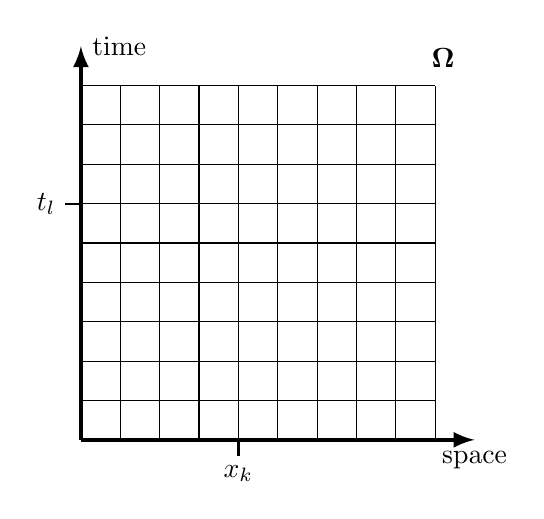
\begin{tikzpicture}
	% Draw the grid
	\tikzset{help lines/.style={color=black}}
	\draw[thin,step=0.5cm,help lines] (0,0) grid (4.5,4.5);
	
	% draw little line to indicate 
	\foreach \x in {2} {     % for x-axis
		\draw [thick] (\x,0) -- (\x,-0.2);
	}
	\foreach \y in {3} {   %% for y-axis
		\draw [thick] (0,\y) -- (-0.2,\y);
	}
	% draw label
	\foreach \x in {2} { \node [anchor=north] at (\x,-0.2) {$x_k$}; }
	\foreach \y in {3} { \node [anchor=east] at (-0.2,\y) {$t_l$}; }
	
	%\foreach \x in {0} { \node [anchor=north] at (\x,-0.2) {$(x_0, 0)$}; }
	\foreach \x in {4.6} { \node [anchor=north] at (\x,5.1) {$\mathbf{\Omega}$}; }
	
	% Draw axes
	\draw[ultra thick,-latex] (0,0) -- (5,0) node[below] {space};
	\draw[ultra thick,-latex] (0,0) -- (0,5) node[right]{time};
	% the co-ordinates -- major
	
	% the co-ordinates -- minor
	\end{tikzpicture}
	
\end{figure}

where one has $n+1$ points in space and $m+1$ points in time. The tuples $(x_k, t_l)$ are then organized in the following manner, the $i$-th entry references $i = (n+1) \cdot l + k$. That is we first label all elements of a certain time step before moving on to the next time step which will then be assembled into one overall system. Details of how this is done will follow in the implementation section. %For simplicity we will only consider equidistant grids in each direction, where $h_t$ denotes the size (better word?) of a mesh cell in time direction and $h_{x_i}$ denote the size in the respective space dimension.

\section{Iterative Methods for Nonlinear Systems}

Our original problem (1.1) is as mentioned before potentially nonlinear, but so far we have only been discussing ways of how to discretise linear problems. Let us therefore now undertake a short excursion of how to solve non-linear problems, which in each iteration step will include solving linearisations that are of the beforementioned type. We assume that we can write the nonlinear problem in the subsequent form and are therefore interested in solving questions of the following type 

\begin{ceqn}
	\begin{align}
	\text{Find } s \in \Omega \subset \mathbb{R}^m \text{ such that } J(s) = 0. 
	\end{align}
\end{ceqn}
for some $J: \Omega \subset \mathbb{R}^m \rightarrow \mathbb{R}_{\geq 0}$. Since this describes a very broad class of problems there are of course many different approaches of how to tackle this question. Here we will introduce three well-known possibilities, gradient descent, and Newton's method, as well as a combination of the two in the form a trust region method. 


\subsection{Gradient Descent Methods}
The method of gradient descent is a computationally inexpensive iterative optimisation algorithm used to find a local minimum of a function $J$. We only have to require that the function $J$ is differentiable in a neighbourhood of each current iterate $s_k$. After an initial guess $s_0$ is chosen, one takes a step in the direction of the negative gradient of $J$ at $s_0$, that is the direction of steepest descent. The iteration then looks as follows 
\begin{ceqn}
	\begin{align}
	s_{k+1} = s_k + \alpha_k (- \nabla J(s_k))
	\end{align}
\end{ceqn}
If the scaling parameter $\alpha_k > 0 $ is chosen sufficiently small, we know that $J(s_{k-1}) \geq J(s_{k})  \geq J(s_{k+1})$. If $ || \nabla J(s_k) || = 0$ we have found a local minimum and hence $s_{k+1} = s_k$. There are a number of strategies that try to select a suitable value for $\alpha_k$, one of them is for example a line search algorithm using the Wolfe conditions \cite{NoceWrig99}.
\smallskip
\\
Under the assumption that $J \in C^1(\Omega)$, bounded and convex and particular choices for the $\alpha_k$, e.g. using an above mentioned line search, the method is guaranteed to converge to a local minimum which is due to the convexity of $J$ the unique global minimiser. However the speed of convergence is dependent on the condition number of the linearised hessian, and can therefore be extremely low if the condition number is high, even when performing an exact line search in every step. Consequently for inexact line search algorithms we cannot expect better convergence rates, and sometimes even have poor convergence rates for relatively well-conditioned problems \cite{NoceWrig99}. Gradient Descent represents a first-order Taylor approximation of $J$ in $s_k$ and gives an updated solution based on this local linear model. A more sophisticated approach than this is for example Newton's method which uses a second order Taylor approximation. 

\subsection{Newton's Method}
It is one of the most well-known and most commonly used methods to solve non-linear problems of the above type \cite{briggs2000multigrid}. Let $J \in C^2(\Omega)$, and hence if differentiate both sides of the equation $J(s) = 0$, we obtain $\nabla J(s) =  [0, 0, ..., 0]^T$, for which we would like to determine the unknown root $s$. We consider a Taylor series expansion for an initial guess $s_0$
\begin{ceqn}
\begin{equation}
\begin{aligned}
\nabla J(s_0 + h) = \nabla J(s_0) + \nabla^2 J(s_0) \cdot h + o(||h||^2), \quad s_0 \in \Omega.
\end{aligned}
\end{equation}
\end{ceqn}
If we now neglect the higher order terms, setting $\nabla J(s_0+h) = 0$ and replacing it by its first order Taylor approximation $\nabla J(s_0) + \nabla^2 J(s_0) \cdot h$, which we can then solve for $h$, under the assumption that $\nabla^2 J(s_0)$ is non-singular and use the result to update our initial guess $s_0$.  One ends up the with iteration 

\begin{ceqn}
\begin{equation}
\begin{aligned}
s_{k+1} = s_k - [\nabla^2 J(s_k)]^{-1} \nabla J (s_k). 
\end{aligned}
\end{equation}
\end{ceqn}

In the case of $J$ being convex and a few additional conditions one can achieve a quadratic rate of convergence for Newton's method compared to a linear one for the method of gradient descent. However except for the one-dimensional case, it is usually very hard or impossible to know if these conditions are actually fulfilled \cite{deuflhard2011newton}. And in addition to the gradient of $J$, one also has to compute the inverse of the Hessian of $J$ in each iteration. For larger systems this is in most cases a rather difficult and computationally expensive problem, which in our case we will try to tackle using a multigrid method [see chapter 5]. 
\smallskip
\\
Hence, a quadratic approximation to find a minimiser only makes sense for a locally convex neighbourhood, otherwise the Newton iteration might not lead to a decrease but instead an increase in energy as it might take an iteration step towards a local maximum. Therefore in order to make use of the faster rate of convergence in convex neighbourhoods of $J$ it makes sense to use a Newton iteration, while in non-convex neighbourhoods it can be preferrable to use a gradient descent step as it is guaranteed to not increase the value of the functional. One option to combine these two is by using a trust region algorithm which has an additional important parameter, the so-called trust region radius and will be introduced in the following section.

\subsection{Trust Region Methods}

Trust region methods is a generic term that comprises globalisation strategies to approximate minima of potentially non-convex optimisation problems. The objective function $J$ is approximated using a model function in a subset of the domain, the so-called trust region. If the model function seems to be a good local fit to the function, the size of the region is expanded, if it is not, the size of the region is reduced. The fit of the model is assessed by comparing the ratio $\rho_k$ of the expected reduction of the objective function by the model and the actual reduction of the function. 
\smallskip
\\
A typical iteration step $k$ can be described in the following way. We have a current trust region that is usually defined as a spherical area of radius $\Delta_k$ and a model function $m_k(p)$ that is supposed to locally approximate $J$ and where $p$ describes the update to the current solution, that is the new step to be taken. We therefore want to solve for $p$, hence we minimise over $p$ within the trust region radius to obtain a solution $p_k$ and can thus determine $\rho_k$, the ratio of the expected compared to the actual reduction. Depending on its value and the parameter thresholding we either reduce $\Delta_k$ if the approximation does not seem like a good fit, and then solve $m_k$ again for $p$ with a smaller $\Delta_{k+1}$. Otherwise we either enlarge it, if $|| p_k || = \Delta_k$, i.e. it is maximal or else leave it the same. If $\rho_k$ is not too small we compute the new solution $s_{k+1} = s_k + p_k$. 
\smallskip
\\
There are many options what to choose as a model function. Among the simplest approaches is the Cauchy point calculation that stems from gradient descent, other popular ones include steihaug's method or the so-called dogleg method \cite{NoceWrig99}. The former uses a conjugate gradient method for a quadratic model function and the later includes a mixture of using information of the first and second derivative of $J$, which is what we used and which will be explained in more detail in the chapter on the implementation [see 6.6.3].
 
\end{document}